\documentclass[a4paper,11pt]{article}

\usepackage{amsmath}
\usepackage{amssymb}

% for proofs  environment
\usepackage{amsthm}

\usepackage[backend=bibtex]{biblatex}
\bibliography{slides6}

% for probability trees
\usepackage{tikz}
\usetikzlibrary{trees}

% for Venn diagrams
\usetikzlibrary{shapes,backgrounds}
% for plots
\usepackage{ pgfplots}
% inserted on suggestion in warning during compilation
\pgfplotsset{compat=1.9}

%for strikethrough text
\usepackage{soul}

%for R source code listing
\usepackage{listings}

%for block quotes
\usepackage{csquotes}

% For not indenting the first line of paragraphs:
\setlength{\parindent}{0pt}
% define the title
\author{John Hancock}
\title{MIT Introduction to Statistics 18.05 Reading 6A Think Questions }
\begin{document}
% generates the title
\maketitle
% insert the table of contents
\tableofcontents
\section{References and License}
We are answering questions in the material from MIT OpenCourseWare
course 18.05, Introduction to Probability and Statistics.

In this document we are answering questions Orloff and Bloom ask in
\cite{slides6}.

We use material in \cite{cubeRoot}, \cite{bold}, \cite{charList}
to write the \LaTeX code for this
document.

Please see the references section for detailed citation information.

The material for the course is licensed under the terms at
\url{http://ocw.mit.edu/terms}.



\section{Questions about X}

In this section we answer questions Orloff and Bloom ask in \cite{reading6a}
regarding a random variable $X$.

Orloff and Bloom specify that $X$ is defined on $\left[ 0, 1 \right]$, and
the pdf of $X$ is $cx^2$.

\subsection{Value of $c$}

Orloff and Bloom ask us to calculate the value of $c$.  We will use rules
and properties for integration from \cite{basicInt} in order to calculate
the value for $c$.

We know
\begin{equation}
  \int_0^1 cx^2 \, dx = 1.
\end{equation}

Therefore
\begin{equation}
  c \int_0^1 x^2 \, dx = 1.
\end{equation}

The anti-derivative of $x^2$ is $\frac{x^3}{3} +C$, so we can replace the
integral in the equation above with:

\begin{equation}
  c \left(\frac{x^3}{3} \bigg\rvert_0^1 \right)=1.
\end{equation}

We then evaluate the anti-derivative over the interval $\left[0, 1\right]$ to
obtain:

\begin{equation}
  c \left(\frac{1^3}{3} \right)=1.
\end{equation}

This implies $c=3$.

\subsection{Mean, variance, and standard deviation of $X$}
\subsubsection{Mean of $X$}
We use the definition of mean value that Orloff and Bloom give in
\cite{reading6a}.
The mean value of $X$ is
\begin{equation}
\mu = \int_0^1 x\left( 3x^2 \right)\,dx.
\end{equation}

We multiply the terms in the polynomial in the integral above to get:

\begin{equation}
\mu = \int_0^1 \left( 3x^3 \right)\,dx.
\end{equation}

We replace the integral above with its anti-derivative:

\begin{equation}
\mu = \frac{3x^4}{4} \bigg\rvert_0^1.
\end{equation}

We evaluate the anti-derivative over the closed interval $\left[0, 1 \right]$ to
find the value of the mean of $X$:

\begin{equation}
\mu = \frac{3}{5}-\frac{18}{16}+\frac{27}{48}\frac{3}{4}.
\end{equation}

\subsubsection{Variance of $X$}
We use the definition of the variance of a continuous random variable in
\cite{reading6a} to compute the variance of $X$.

The definition of Variance Orloff and Bloom give in \cite{reading6a}:

\begin{equation}
  \text{Var}\left(X \right) = E\left( \left( X-\mu\right)^2\right).
\end{equation}

We use the values for $c$ and $\mu$ that we find above to find:
\begin{equation}
  \text{Var}\left(X\right)=\int_0^1 x^{2}3\left(x-\frac{3}{4}\right)^2 \,dx.
\end{equation}

Now we multiply some of the factors in the polynomial in the integral above
to get:

\begin{equation}
  \text{Var}\left(X\right)=\int_0^1 x^{2}3\left(x^2-\frac{6x}{4}+\frac{9}{16}\right) \,dx.
\end{equation}


We continue multiplying factors:

\begin{equation}
  \text{Var}\left(X\right)=\int_0^1 3x^4-\frac{18x^3}{4}+\frac{27x^2}{16} \,dx.
\end{equation}


Now we replace the integral above with its anti-derivative:

\begin{equation}
  \text{Var}\left(X\right)= \frac{3x^4}{5}-\frac{18x^4}{16}+\frac{27x^3}{48} \bigg\rvert_0^1.
\end{equation}

And, we evaluate the anti-derivative over  the interval $\left[0, 1\right]$:

\begin{equation}
  \text{Var}\left(X\right)= \frac{3}{5}-\frac{18}{16}+\frac{27}{48}=\frac{3}{5}-\frac{18}{16}+\frac{9}{16}.
\end{equation}

Now we simplify the expression above further:

\begin{equation}
  \text{Var}\left(X\right)= \frac{3}{5}-\frac{18}{16}+\frac{9}{16}=\frac{3}{5}-\frac{9}{16}=\frac{48}{80}-\frac{45}{80}=\frac{3}{80}.
\end{equation}

Therefore the variance of $X$ is $\frac{3}{80}$.

\subsubsection{Standard Deviation of $X$}

The standard deviation of $X$ is the square root of its variance \cite{reading6a}.  Therefore the standard deviation of $X$ is:

\begin{equation}
\sigma=\sqrt{\frac{3}{80}} \approx
  0.194.
\end{equation}

\subsubsection{Median value of $X$}
The median value of $X$ is the 0.5
quantile of the cdf of $X$
\cite{reading6a}.

In the first part of this problem,
we find that the pdf of $X$ is
$3x^2$.

Therefore we must solve the equation:
\begin{equation}
\int_0^a 3x^2 \,dx = 0.5
\end{equation}

We replace the integral in the
equation above with its
anti-detivative:

\begin{equation}
\frac{3x^3}{3} \bigg\rvert_0^a=0.5.
\end{equation}

And, we evaluate the anti-derivative
above over the interval $\left[0,a
\right]$:

\begin{equation}
\frac{3a^2}{3}=0.5.
\end{equation}

Now it is a matter of doing some
algebra to solve for $a$:

\begin{equation}
3a^2=0.5 \times 3.
\end{equation}

This implies:
\begin{equation}
a^3=0.5.
\end{equation}

Therefore, the median value of $X$ is
$\sqrt[3]{0.5} \approx 0.794$.

\subsection{Standard Deviation of
copies}

For this part of the problem, Orloff
and Bloom give us a set of
random variables $X_1, X_2, \ldots,
X_16$ that are independent, identically-
distributed copies of $X$.
They go on to define $\bar{X}$ as the
average of $X_1, X_2, \ldots, X_16$.

Orloff and Bloom then ask us for the
standard deviation, $\sigma$, of
$\bar{X}$.

$X_1, X_2, \ldots, X_16$ are independent identically-distrubted random
variables.  In \cite{reading6b} Orloff and Bloom show that,for two independent
random variables $X$ and $Y$, $\text{Var}\left( X + Y \right) =
\text{Var}\left( X \right) + \text{Var}\left( Y \right)$.

$\bar{X}$ is the average of $X_1, X_2, \ldots, X_16$.  Therefore

\begin{equation}
\bar{X} = \frac{X_1}{16} + \frac{X_2}{16} + \ldots + \frac{X_{16}}{16}
\end{equation}

We repeatedly apply the result on the sum of variances of random variables
we quoted from \cite{reading6b} above to get

\begin{equation} \label{varsum1}
\text{Var}\left(\bar{X}\right) = \text{Var}\left(\frac{X_1}{16}\right)
 + \text{Var}\left(\frac{X_2}{16}\right) + \ldots +
 \text{Var}\left(\frac{X_{16}}{16}\right).
\end{equation}

In \cite{reading6a} Orloff and Bloom state that for
a continuous random variable $Z$,
Var$\left(aZ + b \right)=a^2\text{Var}\left(Z\right)$.

Therefore we may rewrite equation \ref{varsum1} as
\begin{equation} \label{varsum2}
\text{Var}\left(\bar{X}\right) = \frac{1}{16^2}\left(\text{Var}\left(X_1\right)
 + \text{Var}\left(X_2\right) + \ldots +
 \text{Var}\left(X_16\right)\right).
\end{equation}

For this problem, Orloff and Bloom give us that
$X_1 , X_2 , \ldots , X_16$ are identical copies
of $X$, so the variances of $X_1 , X_2 , \ldots , X_16$
are all equal to the variance of $X$.

We computed the variance of $X$ above.
$\text{Var}\left(X \right)=\frac{3}{80}$.

This implies that

\begin{equation}
\text{Var}\left(\bar{X}\right) = \frac{16}{16^2}\left(\frac{3}{80}\right).
\end{equation}

Hence the standard deviation of $\bar{X}$ is
\begin{equation}
\sigma_{\bar{X}} = \sqrt{\frac{3}{80\times16}} \approx 0.0484.
\end{equation}

\subsection{PDF of function of X}
Orloff and Bloom ask us to let $Y=X^4$, and ask us to find the pdf of $Y$.

Let $F_y$ be the cdf of $Y$. Then:

\begin{equation} \label{pofY}
  P\left(Y < y \right) = P \left( X^4 < y \right).
\end{equation}

For $y \neq 0$, equation \ref{pofY} is true if, and only if

\begin{equation} \label{pofY2}
  P\left(Y < y \right) = P \left( X < \sqrt[4]{y} \right).
\end{equation}

The cdf of $X$ is $x^3$. Furthermore, the cdf of $X$ is defined on
the interval $\left[0, 1 \right]$ so equation \ref{pofY2} holds if,
and only if:

\begin{equation}\label{pofY3}
  P\left(Y < y \right) = x^3 \bigg\rvert_0^{\sqrt[4]{y}}.
\end{equation}

We can evaluate equation \ref{pofY3} over the interval
$\left[ 0, \sqrt[4]{y} \right]$; therefore, equation \ref{pofY3} is
true if, and only if:


\begin{equation}\label{pofY4}
  P\left(Y < y \right) = \left( \sqrt[4]{y}\right)^3 .
\end{equation}

Equation \ref{pofY3} is true if, and only if, the cdf of $Y$ is
$\left( \sqrt[4]{y} \right)^3$.

The pdf is the derivative of the cdf, therefore the pdf of $Y$ is:
$\frac{3}{4} y^{\frac{-1}{4}}$

\section{Histograms}
We use R-studio in order to draw the histograms for this list of numbers:

$1$, $1.2$, $1.3$, $1.6$, $1.6$, $2.1$, $2.2$, $2.6$, $2.7$, $3.1$, $3.2$,
$3.4$, $3.8$, $3.9$, $3.9$

We rely on the examples in \cite{studio3r}  in order to create the histograms
below.
\subsection{Equal bin widths of 0.5}
\subsubsection{Frequency Histogram}

The R code we write to generate the image below is:

\begin{lstlisting}
binwidth = .5;
data = c(1, 1.2, 1.3, 1.6, 1.6, 2.1, 2.2, 2.6, 2.7, 3.1, 3.2, 3.4, 3.8, 3.9, 3.9);
bins = seq(0, 4, 0.5)
hist(data, breaks=bins, col='red', freq=TRUE)
\end{lstlisting}

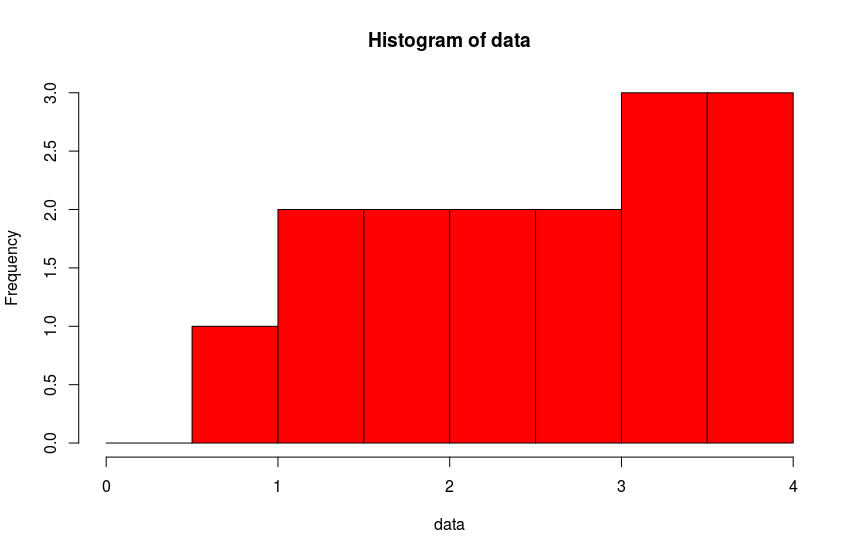
\includegraphics[scale=0.5]{freq-hist-1}

\subsubsection{Density Histogram}

The R code to generate the image below is:

\begin{lstlisting}
binwidth = .5;
data = c(1, 1.2, 1.3, 1.6, 1.6, 2.1, 2.2, 2.6, 2.7, 3.1, 3.2, 3.4, 3.8, 3.9, 3.9);
bins = seq(0, 4, 0.5)
hist(data, breaks=bins, col='yellow', freq=FALSE)
\end{lstlisting}

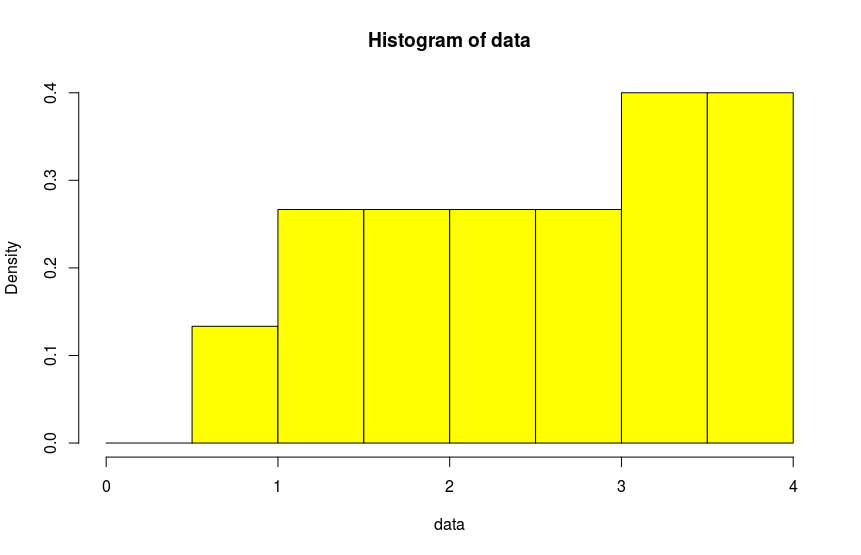
\includegraphics[scale=0.5]{dens--hist-1}


\subsection{Unequal bin widths}

\subsubsection{Frequency Histogram}

The R code we write to generate the image below is:

\begin{lstlisting}
binwidth = .5;
data = c(1, 1.2, 1.3, 1.6, 1.6, 2.1, 2.2, 2.6, 2.7, 3.1, 3.2, 3.4, 3.8, 3.9, 3.9);
bins = c(0,1,3,4)
hist(data, breaks=bins, col='blue', freq=TRUE)
\end{lstlisting}

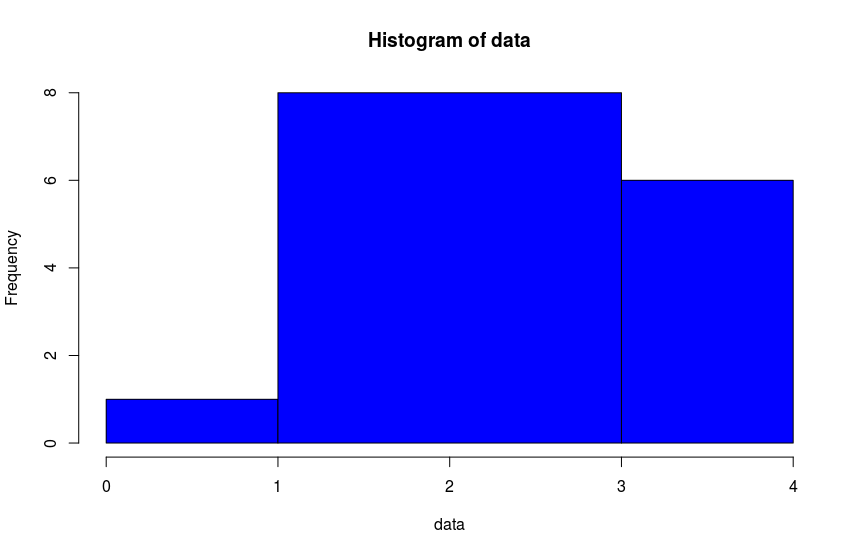
\includegraphics[scale=0.5]{freql-unequal-hist.png}

\subsubsection{Density Histogram}

The R code we write to generate the image below is:
\begin{lstlisting}
binwidth = .5;
data = c(1, 1.2, 1.3, 1.6, 1.6, 2.1, 2.2, 2.6, 2.7, 3.1, 3.2, 3.4, 3.8, 3.9, 3.9);
bins = c(0,1,3,4)
hist(data, breaks=bins, col='blue', freq=FALSE)
\end{lstlisting}

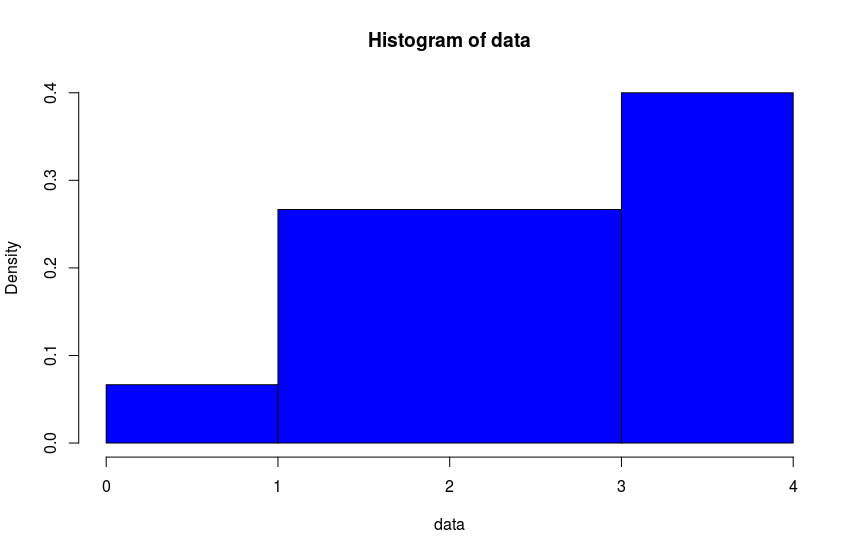
\includegraphics[scale=0.5]{dens-hist-unequal}

\section{Election}
\subsection{Central Limit Theorem}
The first part of the board question that Orloff and Bloom ask
us is a task to carefully write the central limit theorem.

The central limit theorem is:

Suppose $X_1, X_2, \ldots, X_n, \ldots$ are independent identically distributed
random variables each having mean $\mu$, and standard deviation $\sigma$. For
each $n$ let $S_n$ denote the sum and let $\bar{X_n}$ be the average of
$X_1, \ldots, X_n$.
\begin{equation}
  S_n = X_1 + X_2 + \ldots + X_n = \sum_{i=i}^n X_i
\end{equation}

\begin{equation}
  \bar{X_n} = \frac{X_1 + X_2 + \ldots + X_n}{n} = \frac{S_n}{n}
\end{equation}

The properties of mean and variance show: $E\left(S_n\right)=n\mu$,
$\text{Var}\left( S_n \right)=n\sigma^2$, $\sigma_{S_n}=\sqrt{n}\sigma$,
$E\left(\bar{X_n}\right) = \mu$, Var$\left(\bar{X_n}\right)=\frac{\sigma^2}{n}$,
$\sigma_{\bar{X_n}} = \frac{\sigma}{\sqrt{n}}$.

Since they are multiples of each other, $S_n$ and $\bar{X_n}$ have the same
standardization
\begin{equation}
  Z_n = \frac{S_n- \mu}{\sigma\sqrt{n}}
  = \frac{\bar{X_{n}} - \mu}{\frac{\sigma}{\sqrt{n}}}
\end{equation}

\textbf{Central Limit Theorem:} for large $n$,
\begin{equation}
X_n \approx  N\left( \mu, \frac{\sigma^2}{n} \right), S_n \approx N\left(n\mu, n\sigma^2 \right),
  Z_n \approx N \left(0, 1\right)
\end{equation}

\subsection{Poll result probability}
For the second part of the question, Orloff and Bloom ask us to
use the central limit theorem to estimate the probability $p$
that we conduct a poll where we know that 50\% of the population
supports the candidate, but the poll shows that at least 55\% of the population
supports a candidate named Erika.  Orloff and Bloom write that the
population size is $400$ people.

We let $\mathcal{E}$ be the discrete random variable that is equal to the
number of people that say they will vote for Erika when we conduct the poll.

In order to apply the central limit theorem to estimate $p$, we must standardize
$i\mathcal{E}$ \cite{reading6b}, \cite{slides6Sol}.

We model the act of polling one person as a trial of a Bernoulli experiment
\cite{reading6b}. $\mathcal{E}$ is then the sum of the number of Bernoulli
experiments where the person we poll says she or he will vote for Erika.
Then we can apply the central limit theorem because $\mathcal{E}$ is the
sum of independent, identically distributed random numbers.

We are given that the size of the population is $400$ people, and the fraction of
people that vote for Erika is \%50.  Therefore the expected  value, $\mu$ of
$\mathcal{E}$ is $200$.

We use the formula Orloff and Bloom derive in \cite{reading5a} for the
variance of a Bernoulli random variable.  The probability $q$ of one
person we poll saying he or she will vote for Erika is 50\%, so according
\cite{reading5a}, the standard deviation of the Bernoulli random
variable that is 1 if the person says she or he will vote for Erika, and 0
otherwise is $\left(1-0.5 \right) \left(0.5 \right) = 0.25$.  We can
apply the property of variance Orloff and Bloom show \cite{reading5a} that
the variance of the sum of random variables is the sum of the variances of
the terms of the sum to get $\text{Var}\left( \mathcal{E} \right)=0.25 \times 400=100$.
Therefore the standard deviation of $\mathcal{E}$ is $10$.

We have the mean and standard deviation of $\mathcal{E}$, so we can
standardize $\mathcal{E}$:
\begin{equation}
   \frac{\mathcal{E} - 200}{10}.
\end{equation}

If 55\% of the 400 people we poll answer that they will vote for Erika,
then this means that $0.55 \times 400 = 220$ people answer they
will vote for Erika.  So, in this case, $\mathcal{E}=220$.

We wish to use the central limit theorem to esitmate
$P\left( \mathcal{E} \geq 220 \right)$.

The standardized value of $\mathcal{E}$ is:

\begin{equation}
   \frac{220 - 200}{10} = 2.
\end{equation}

So we estimate $P\left(\mathcal{E} \right) \geq 220$ with
$P\left( Z \right) \geq 2$.

We justify that this estimate is valid: recall that $\mathcal{E}$ is the
sum of the outcomes of $400$ independent Berounilli trials, and
that the central limit theorem allows us to approximate such
sums with the standard normal distribution \cite{reading6b}.

We know from the rule of thumb \cite{reading5c} that
$P\left( -2 \leq Z \leq 2 \right) \approx 0.95$.  Therefore the area
under the curve of the probability density function of $Z$,
$\phi$ is 0.95.  We are interested in the value of $P\left(Z \geq 2 \right)$. So
we are interested in the area under the curve where $Z \geq 2$. We know that
the total area under the curve of $\phi$ is 1, and that $\phi$ is
symmetric with respect to the $x$ axis \cite{reading5c}.  Therefore
$P\left(Z \geq 2 \right) \approx \frac{1-0.95}{2} \approx 0.025$.

Therefore the probability of our conducting a poll of 400 people
where at least 55\% of the people answer that they will  vote
for Erika is 0.025.

\subsection{Probability of poll for Ruthi}
In this section we entertain the next question that Orloff
and Bloom ask for candidate Ruthi. All of the conditions
and their consequences that we write about above apply for
this question as well.

Orloff and Bloom give us that 25\% of the population
votes for Ruthi.

We wish to know the probability that, when we conduct a
poll of 400 people, less than 20\% of the people say that
they will vote for Ruthi.

Let the random variable $\mathcal{R}$ be the number of peoplewe  poll that say
they will vote for Ruthi.

We wish to use the central limit theorem to estimate $P\left( \mathcal{R} < 20\% \right)$.

Now the Bernoulli trial where we ask one person who he or she will
vote for has a probability of the outcome where the person says
she or he will vote for Ruthi of $025\%$.  Therefore the mean value, $\mu$
of $\mathcal{R}$ is $100$, and the standard deviation of $\mathcal{R}$ is
$\sqrt{75}$.

We derive the standard deviation and mean of $\mathcal{R}$
in the same way that we derive the standard deviation and mean of
$\mathcal{E}$ in the previous section above.

If less than 20\% of the people we poll answer that they will vote
for Ruthi, then we have $\mathcal{R} < 80$.

We wish to use the central limit theorem to estimate
$P\left(\mathcal R < 80 \right)$.

In order to do so, we standardize $\mathcal{R}$.  The standardized
value of $\mathcal{R}$ in the case where $\mathcal{R} = 80$ is
$\frac{80-100}{sqrt{75}} \approx -2.309$.

Therefore we apply the central limit theorem to estimate
$P \left( \mathcal{R} < 80 \right)$ with
$P \left( Z < -2.309)$. We use the pnorm function in
R to get $P \left( Z < -2.309 \right) \approx 0.010$.

Therefore the probability that we conduct a poll and find that
less than 20\% of the people we poll answer that they
will vote for Ruthi is about one percent.

\printbibliography{}
\end{document}
